% TODO(team): Keep appendix figures tied to their original captions and units.
\section{Appendix}
\begin{frame}{E1: paired effects}
\centering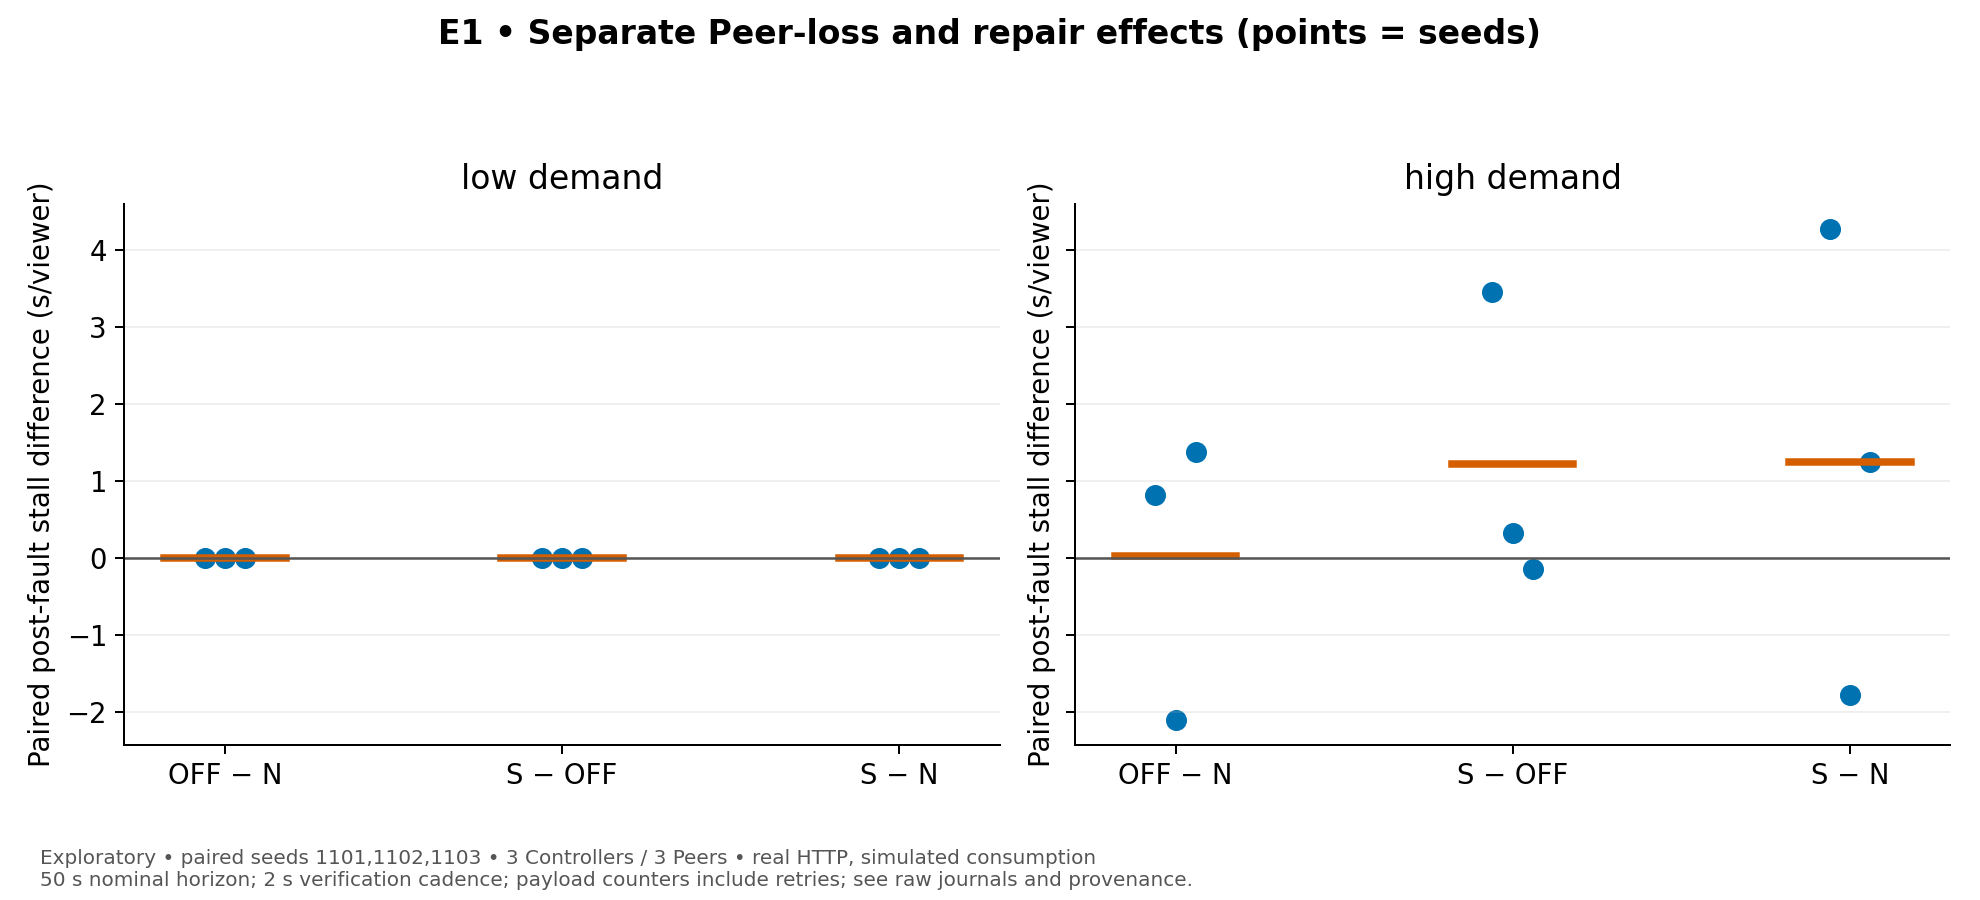
\includegraphics[width=\textwidth,height=.70\textheight,keepaspectratio]{E1-paired-effects.png}
\note{Early failed sessions can report lower observed stalls; show completion alongside this plot. Source: archived E1 paired effects.}
\end{frame}
\begin{frame}{E3: outcomes by failed source capacity}
\centering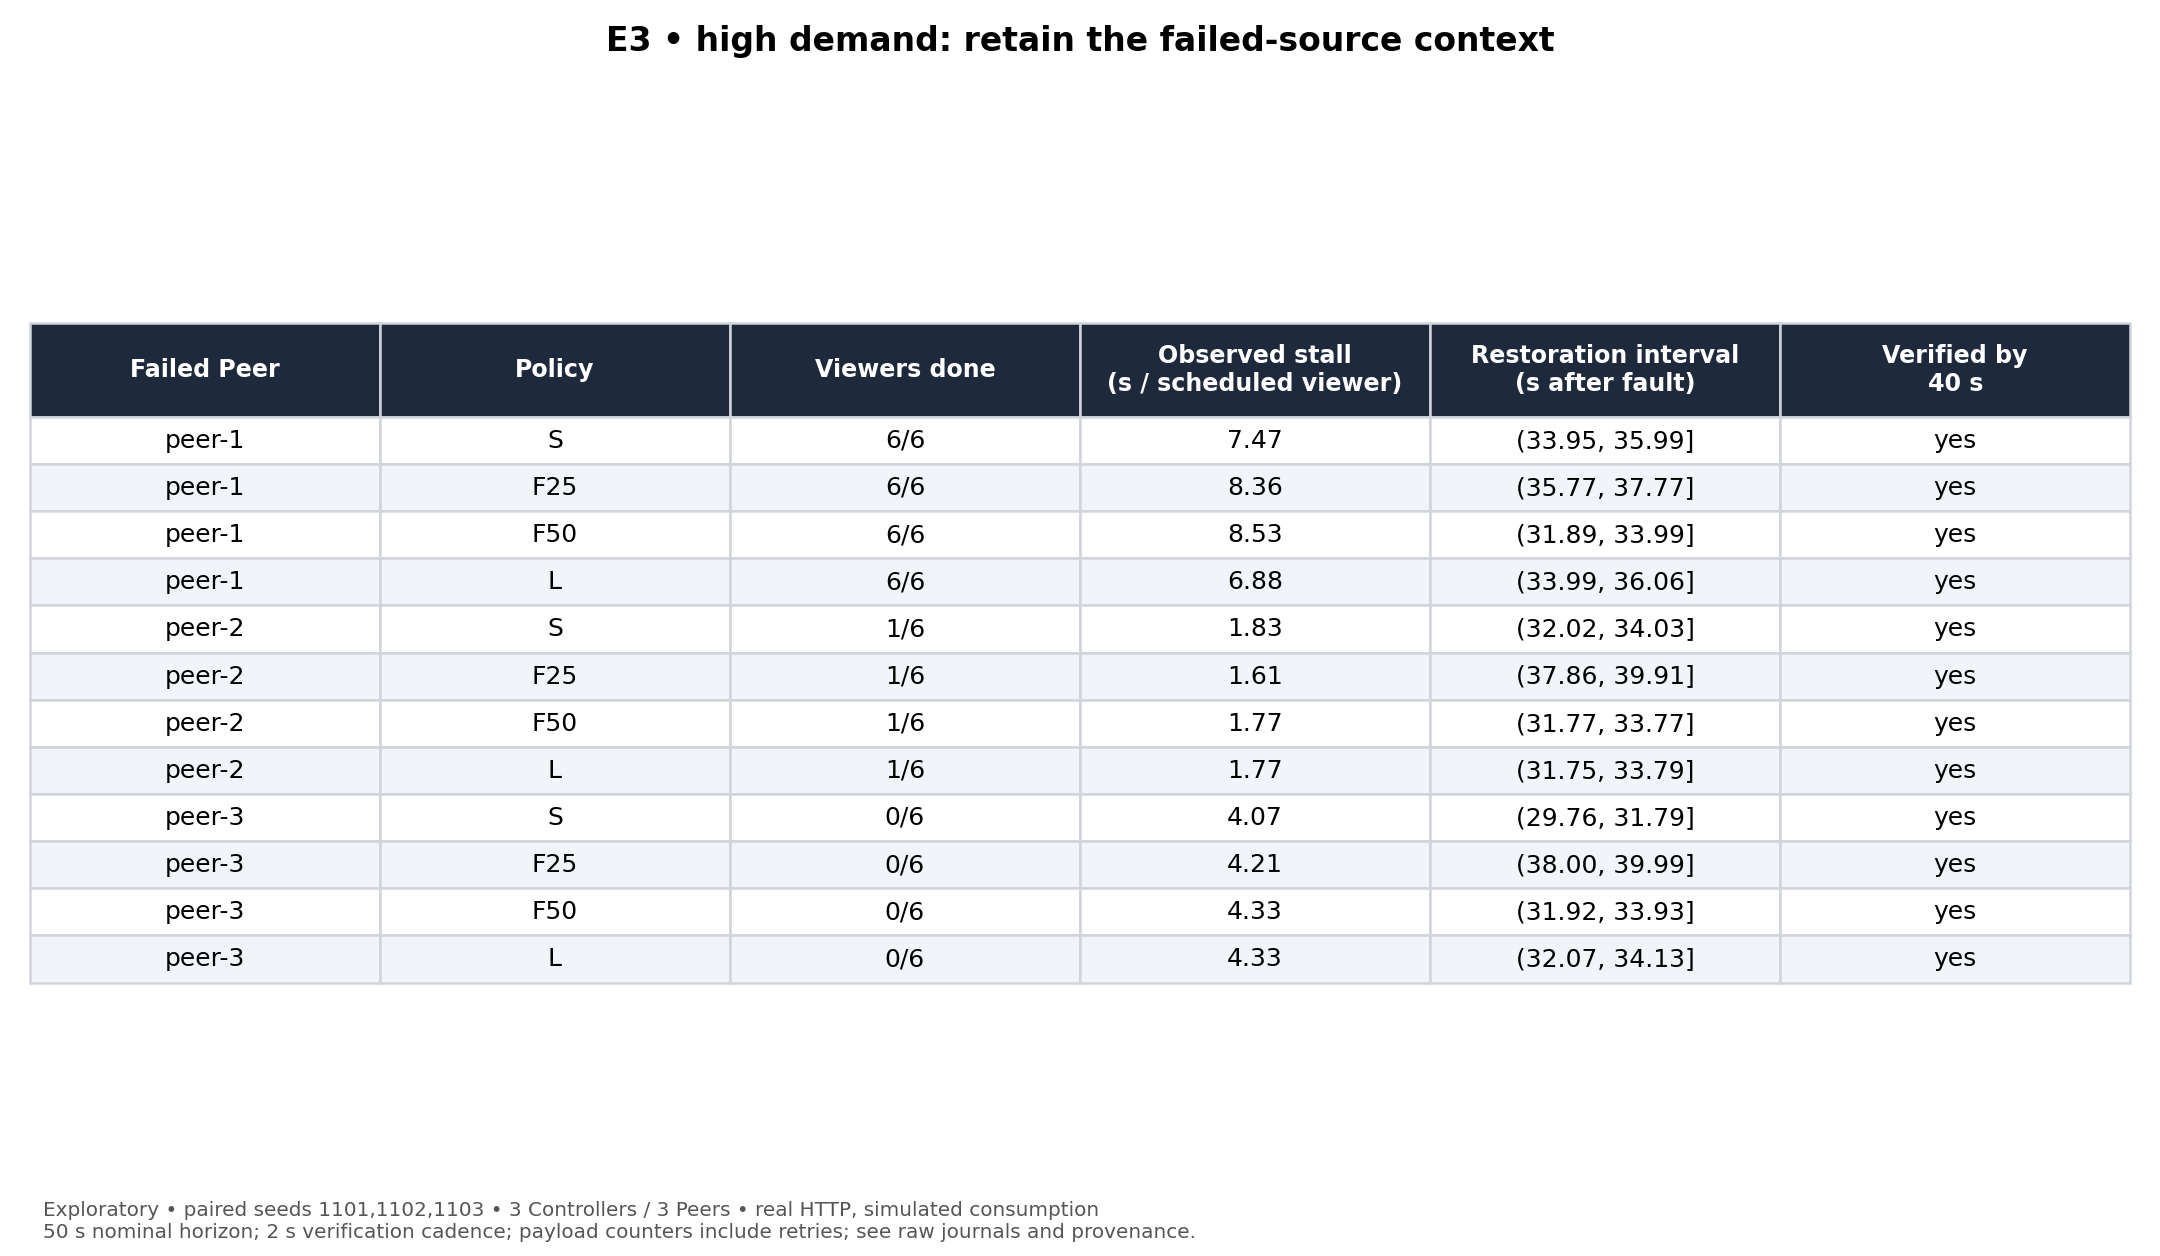
\includegraphics[width=\textwidth,height=.70\textheight,keepaspectratio]{E3-high-by-failed-peer.png}
\note{One paired context per failed capacity. These rows are not repeated capacity-stratum estimates.}
\end{frame}
\begin{frame}{L: recorded repair-budget behavior}
\centering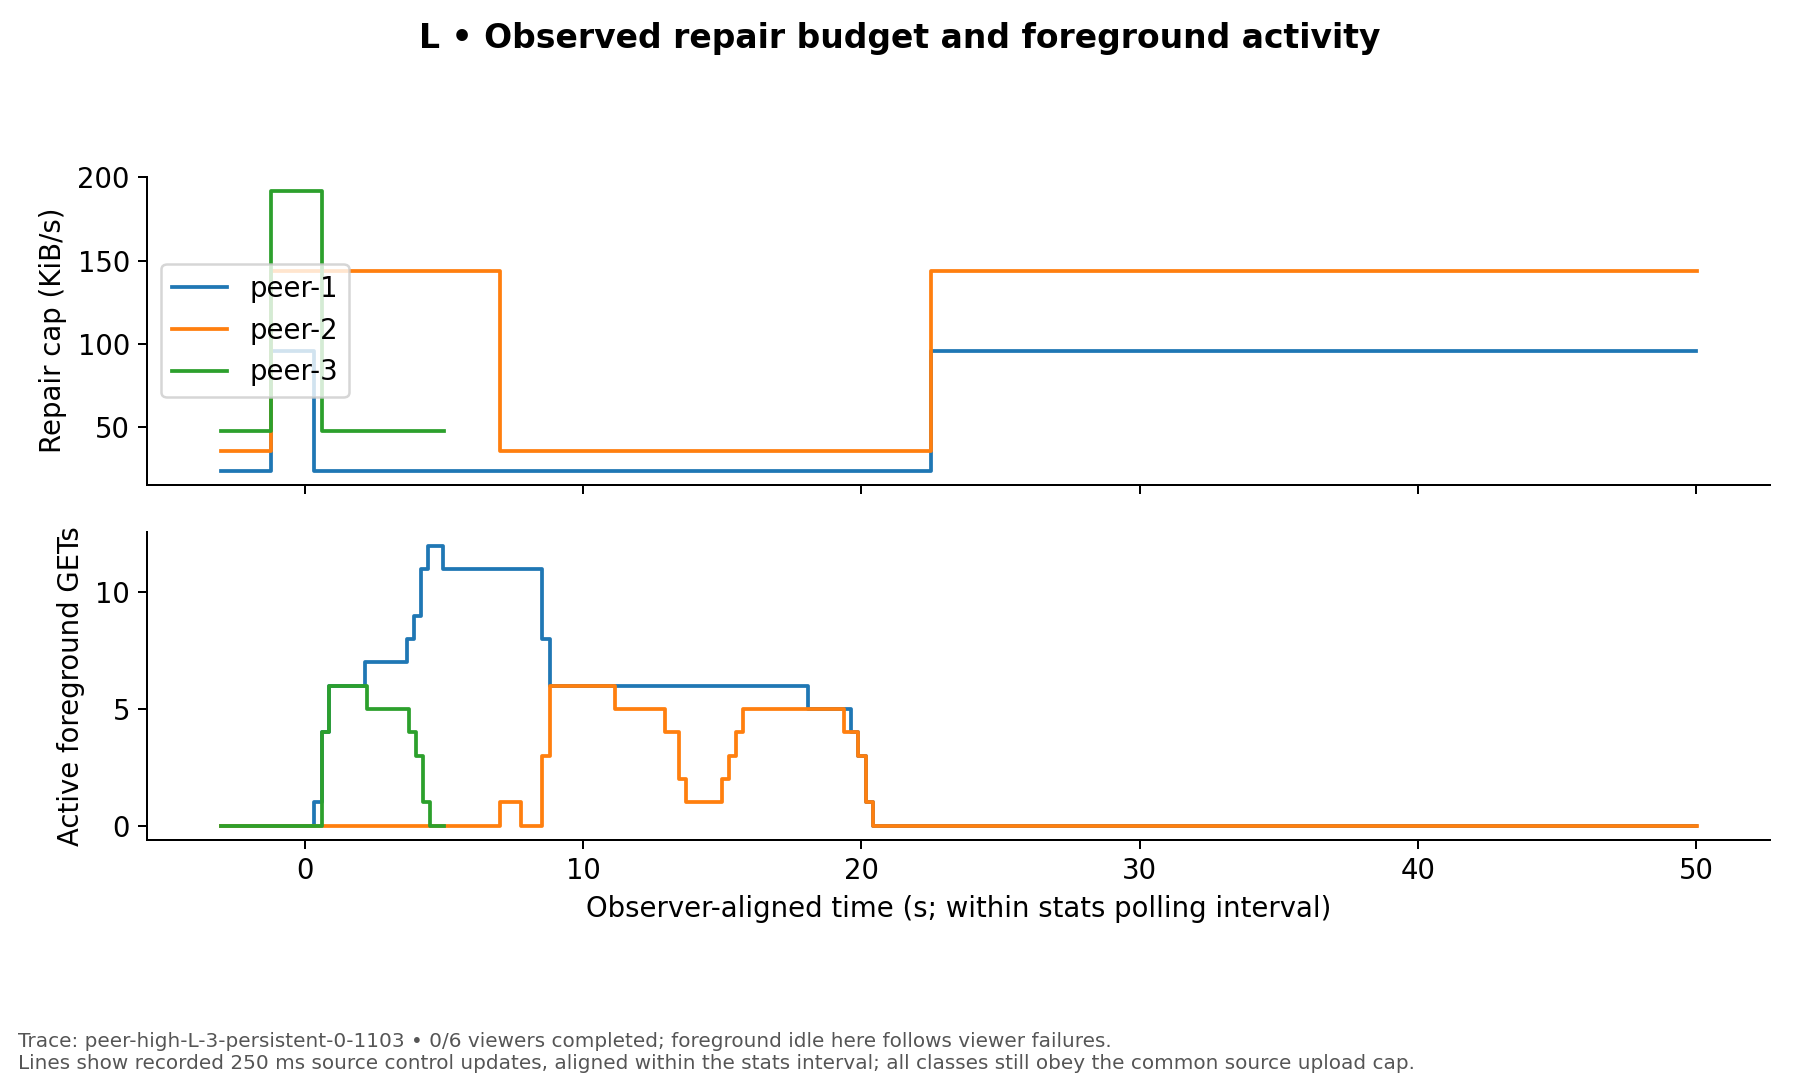
\includegraphics[width=\textwidth,height=.70\textheight,keepaspectratio]{L-budget-trace.png}
\note{This illustrated seed has 0/6 viewer completion. Idle follows failed viewers, not successful playback. The age floor did not activate during the compact performance runs.}
\end{frame}
\begin{frame}{E5: fault-relative recovery distribution}
\centering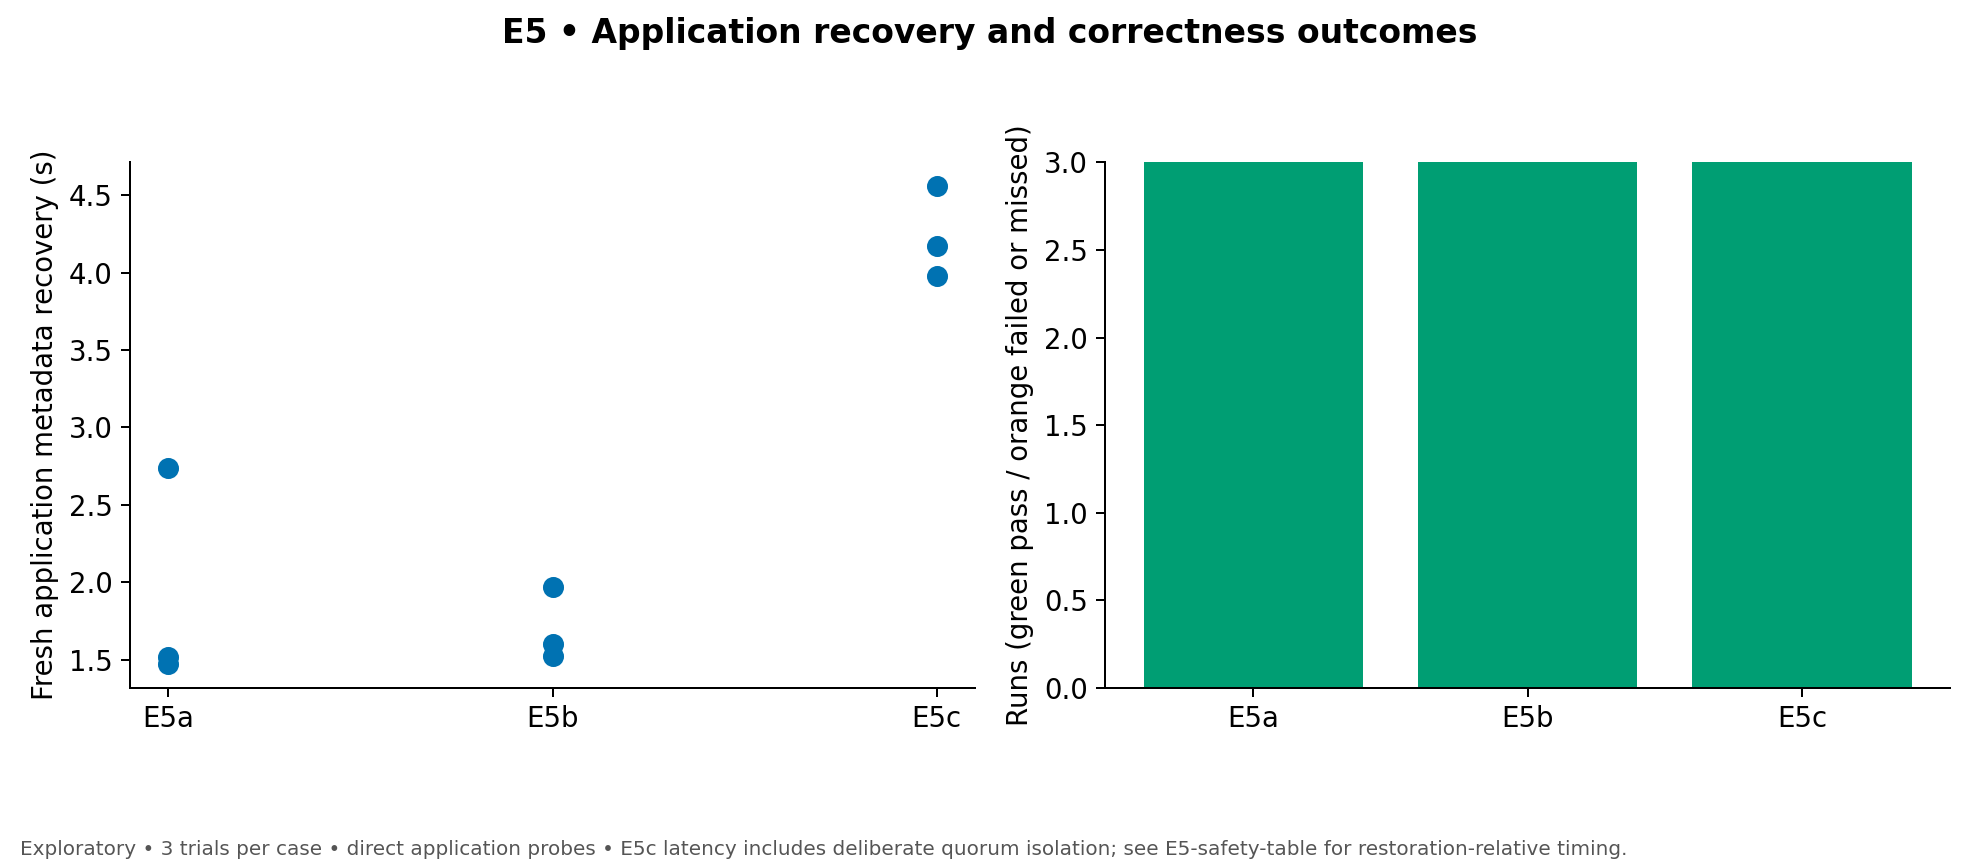
\includegraphics[width=\textwidth,height=.70\textheight,keepaspectratio]{E5-controller.png}
\note{This plot retains deliberate isolation in E5c. The main E5 table instead uses quorum-restoration-relative timing. Do not compare the two timing origins as if identical.}
\end{frame}
